\appendix
\chapter{First Appendix}
\label{app: first}

\noindent List of Packages used:
\begin{itemize}
\label{appendix: pack_list}
    \item DataFrames.jl
    \item Statistics.jl
    \item StatsPlots.jl
    \item StatsBase.jl
    \item LinearAlgebra.jl
    \item TimeSeries.jl
    \item Pkg.jl
    \item PyCall.jl
    \item Conda.jl
    \item Pandas.jl
    \item Plots.jl
    \item KernelDensity.jl
    \item Flux.jl
    \item SciPy.jl
    \item Random.jl
    \item JuMP.jl
    \item DelimitedFiles.jl
    \item SCS.jl
    \item Convex.jl
    \item MathOptInterface
    \item PyPlot.jl
    \item ShiftedArrays.jl
    \item GLM.jl
    \item MLBase.jl
    \item DataFrames.jl
    \item Distributions.jl
    \item MarketTechnicals.jl
    \item Requires.jl
\end{itemize}


\begin{figure}[h]
  \centering
  \subfloat{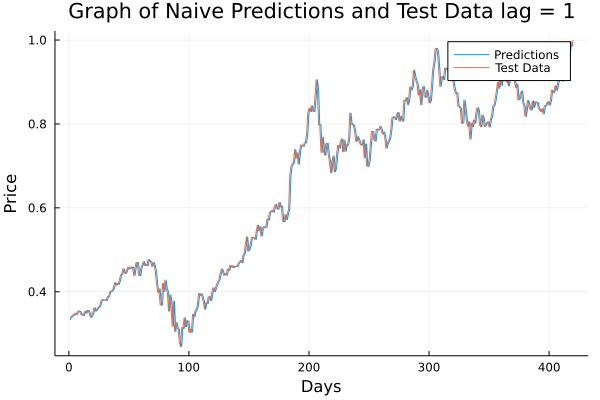
\includegraphics[width=.45\columnwidth]{appendix/simple_machine/lag_app_1.png}}\quad
  \subfloat{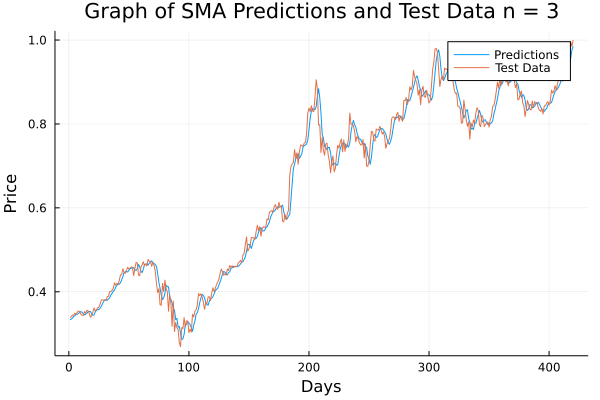
\includegraphics[width=.45\columnwidth]{appendix/simple_machine/sma_app_3.png}}\\
  \subfloat{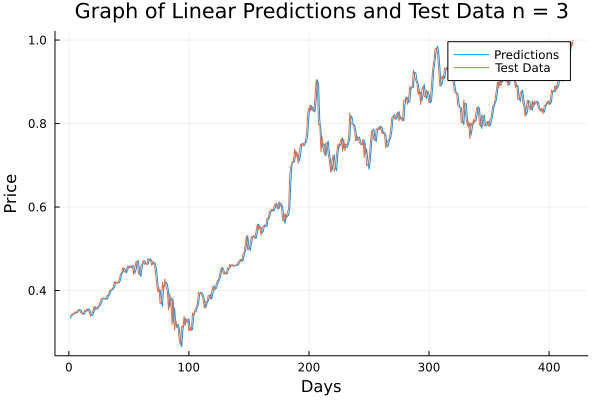
\includegraphics[width=.45\columnwidth]{appendix/simple_machine/lin_app_3.png}}\quad
  \caption{(a)Naive, (b)SMA, (c)Linear}
  \label{fig: full_simple}
\end{figure}

\begin{figure}
    \centering
    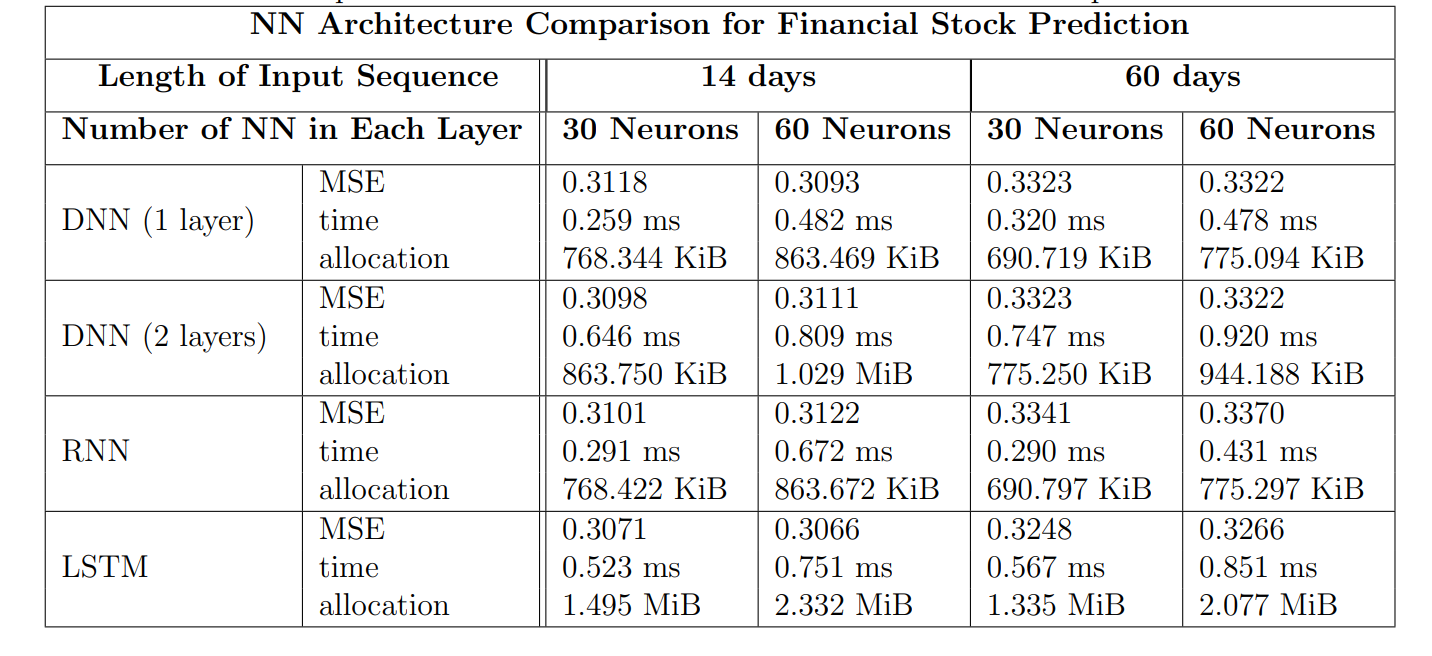
\includegraphics[width=0.9\columnwidth]{appendix/simple_machine/ml_table.PNG}
    \caption{Complete ML Table for variety of Architecture formulations \cite{ml_paper}}
    \label{fig: full_machine}
\end{figure}

\begin{figure}[h]
  \centering
  \subfloat{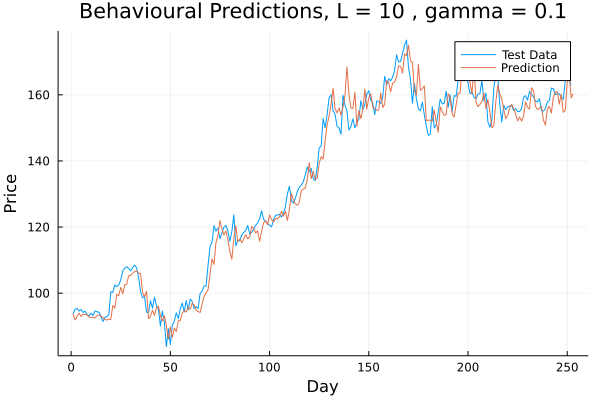
\includegraphics[width=.45\columnwidth]{Results/Simple_vs_Behavioural/depth_10_gamma_1.png}}\quad
  \subfloat{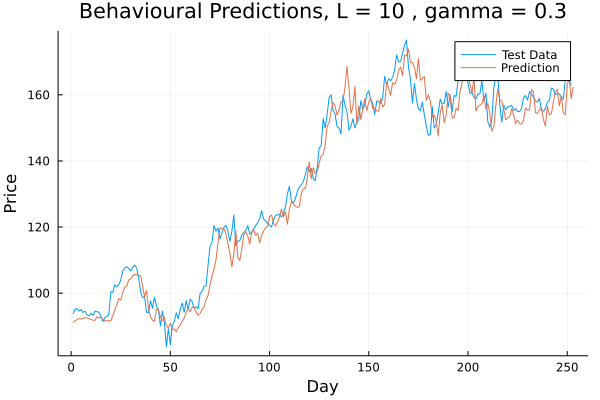
\includegraphics[width=.45\columnwidth]{Results/Simple_vs_Behavioural/depth_10_gamma_2.png}}\\
  \subfloat{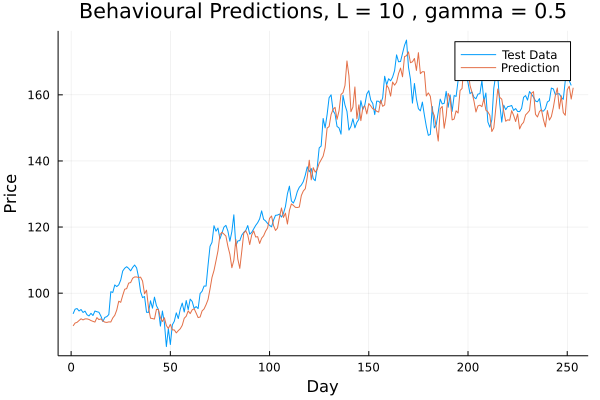
\includegraphics[width=.45\columnwidth]{Results/Simple_vs_Behavioural/depth_10_gamma_3.png}}\quad
  \subfloat{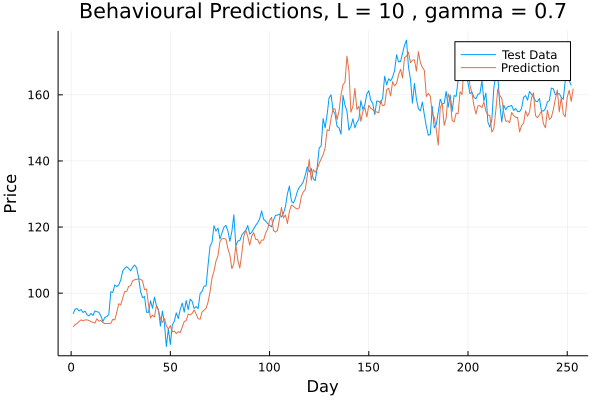
\includegraphics[width=.45\columnwidth]{Results/Simple_vs_Behavioural/depth_10_gamma_4.png}}
  \caption{(a)$L=10$ $\gamma=0.1$, (b)$L=10$ $\gamma=0.3$, (c)$L=10$ $\gamma=0.5$, (d)$L=10$ $\gamma=0.7$}
  \label{fig: behave_full_1}
\end{figure}

\begin{figure}[h]
  \centering
  \subfloat{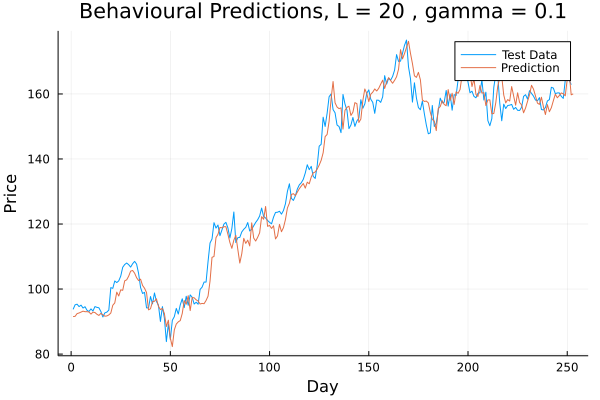
\includegraphics[width=.45\columnwidth]{Results/Simple_vs_Behavioural/depth_20_gamma_1.png}}\quad
  \subfloat{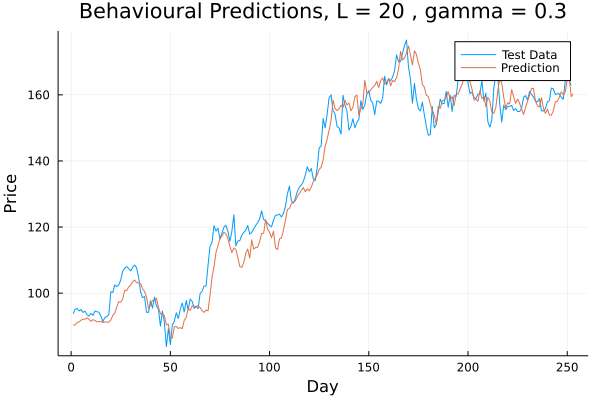
\includegraphics[width=.45\columnwidth]{Results/Simple_vs_Behavioural/depth_20_gamma_2.png}}\\
  \subfloat{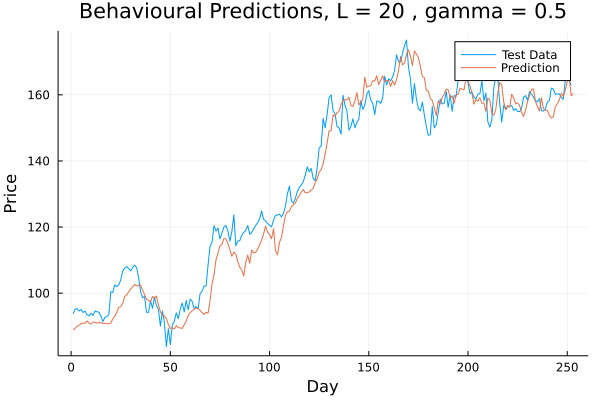
\includegraphics[width=.45\columnwidth]{Results/Simple_vs_Behavioural/depth_20_gamma_3.png}}\quad
  \subfloat{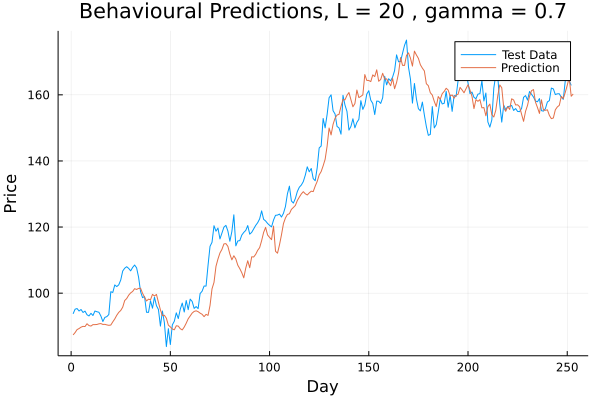
\includegraphics[width=.45\columnwidth]{Results/Simple_vs_Behavioural/depth_20_gamma_4.png}}
  \caption{(a)$L=20$ $\gamma=0.1$, (b)$L=20$ $\gamma=0.3$, (c)$L=20$ $\gamma=0.5$, (d)$L=20$ $\gamma=0.7$}
  \label{fig: behave_full_2}
\end{figure}

\begin{figure}[h]
  \centering
  \subfloat{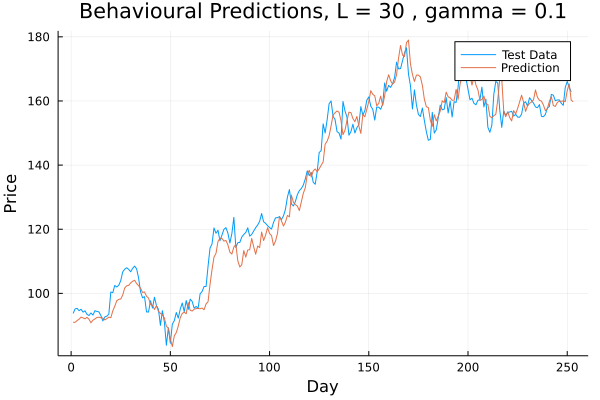
\includegraphics[width=.45\columnwidth]{Results/Simple_vs_Behavioural/depth_30_gamma_1.png}}\quad
  \subfloat{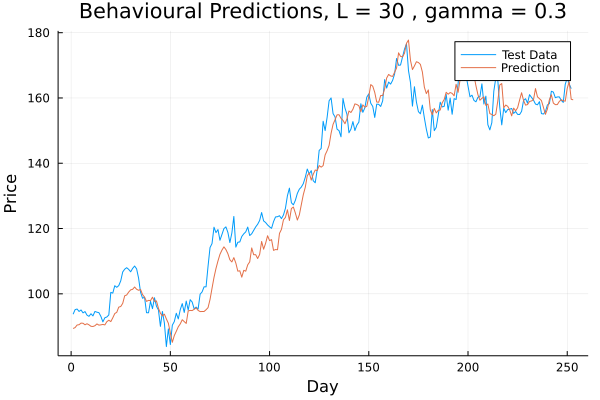
\includegraphics[width=.45\columnwidth]{Results/Simple_vs_Behavioural/depth_30_gamma_2.png}}\\
  \subfloat{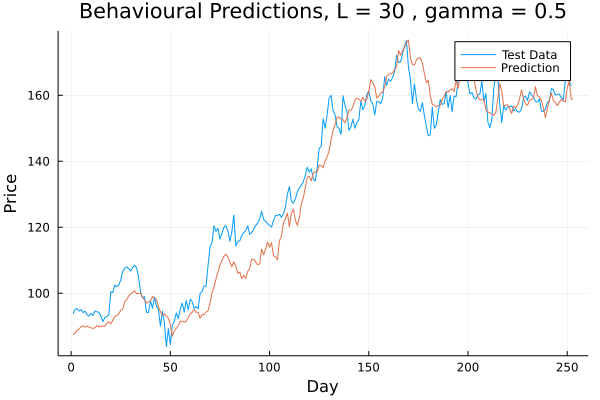
\includegraphics[width=.45\columnwidth]{Results/Simple_vs_Behavioural/depth_30_gamma_3.png}}\quad
  \subfloat{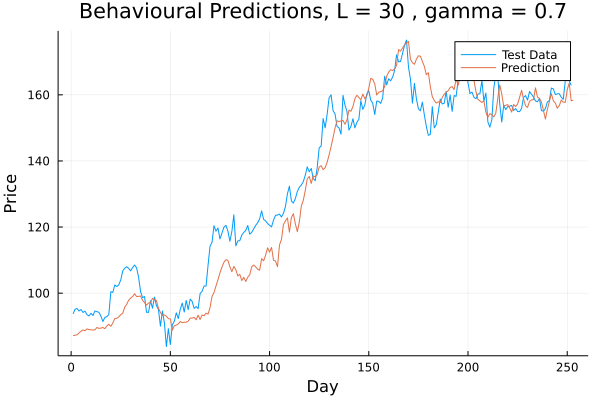
\includegraphics[width=.45\columnwidth]{Results/Simple_vs_Behavioural/depth_30_gamma_4.png}}
  \caption{(a)$L=30$ $\gamma=0.1$, (b)$L=30$ $\gamma=0.3$, (c)$L=30$ $\gamma=0.5$, (d)$L=30$ $\gamma=0.7$}
  \label{fig: behave_full_3}
\end{figure}

\begin{figure}[h]
  \centering
  \subfloat{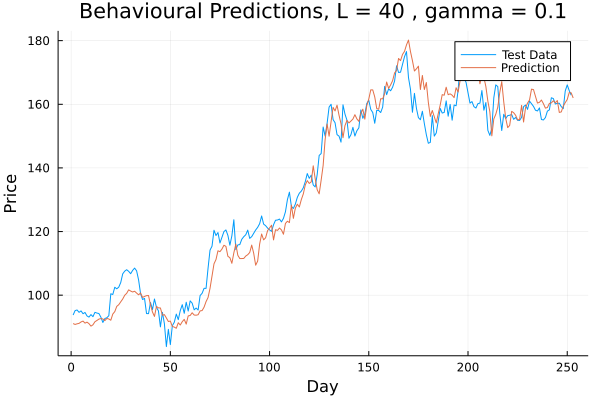
\includegraphics[width=.45\columnwidth]{Results/Simple_vs_Behavioural/depth_40_gamma_1.png}}\quad
  \subfloat{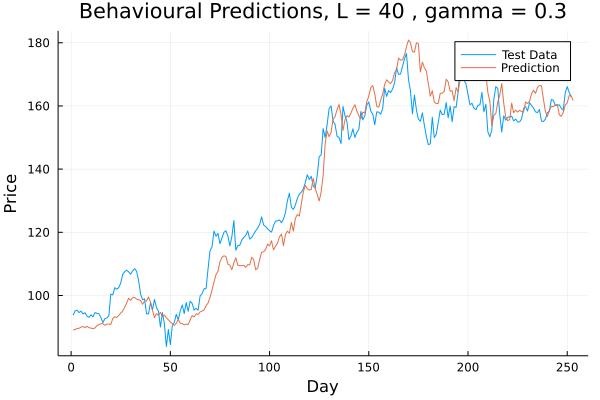
\includegraphics[width=.45\columnwidth]{Results/Simple_vs_Behavioural/depth_40_gamma_2.png}}\\
  \subfloat{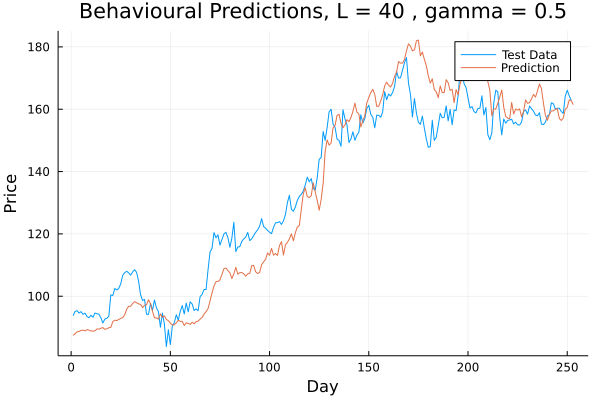
\includegraphics[width=.45\columnwidth]{Results/Simple_vs_Behavioural/depth_40_gamma_3.png}}\quad
  \subfloat{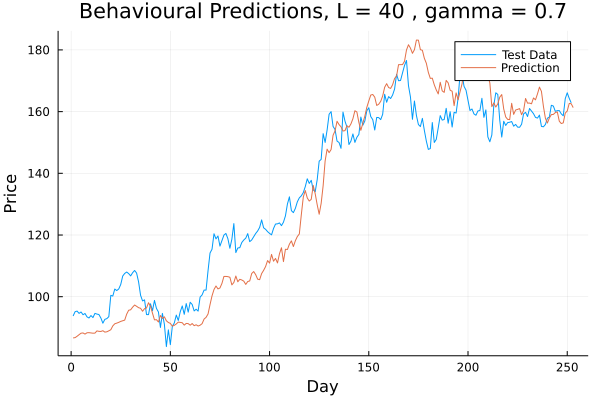
\includegraphics[width=.45\columnwidth]{Results/Simple_vs_Behavioural/depth_40_gamma_4.png}}
  \caption{(a)$L=40$ $\gamma=0.1$, (b)$L=40$ $\gamma=0.3$, (c)$L=40$ $\gamma=0.5$, (d)$L=40$ $\gamma=0.7$}
  \label{fig: behave_full_4}
\end{figure}


\chapter{Code Listings}

\begin{listing}[h]
\caption{Description of Main Functions used in the Data.jl}
\label{lst: Data.jl}
\begin{minted}[mathescape,
              frame=lines,]{julia}
              
function get_data(tickr::String, start::String,
finish::String, range::String, int::String)
    live_data = yfinance.download(tickr, start,
    finish, period = range, interval = int) #import
    data from any period desired
    info = Pandas.DataFrame(live_data) # Wrap in a pandas DataFrame
    info = Pandas.reset_index(info) # set the index 
    info = DataFrames.DataFrame(info) # Convert to julia DataFrame
    Pandas.display(info) # display
    all_data = info
    all_data # return data
end

#standardize a set of data according to mean and std dev of a set of training data
function standardize(data, train) 
    standardized =
    StatsBase.zscore(data,Statistics.mean(train), Statistics.std(train))
    standardized
end

# get_train_data selects the first 2/3 of data from get_data
function split_train_test(df)
    train_data = df[1:floor(Int64,size(df,1)*2/3), :]
    test_data = df[floor(Int64,size(df,1)*2/3)+1:size(df,1),:]
    
    train_data, test_data
end

\end{minted}
\end{listing}



\begin{listing}[h]
\caption{Description of the Main Functions used in Simple.jl}
\label{lst: Simple.jl}
\begin{minted}[mathescape,
              frame=lines,]{julia}

# delays the specified array by a select amount of "delay"

function naive(data::Array, delay::Int)
    predictions = copy(GLM.lag(data, delay))
    predictions
end

# calculates the simple moving average of the
# specified array using an "n" number of points

function sma(a::Array, n::Int)
    vals = zeros(size(a,1)+1, size(a,2))

    for i in 1:size(a,1) - (n-1)
        for j in 1:size(a,2)
            vals[i,j] = mean(a[i:i+(n-1),j])
        end
    end
    predictions = copy(GLM.lag(vals,n))
    predictions
end

# calculates the moving linear prediction of the
# specified array using an "n" number of points
# works similar to the simple moving average
# makes use of the linear_predict function

function linear_prediction(data::Array, n::Int)
    vals = zeros(size(data,1)+1)

    for i in 1:size(data,1) - (n-1)
        vals[i] = linear_predict(data[i:i+(n-1)])
    end
    predictions = copy(GLM.lag(vals,n))
    predictions
end

# calculates the linear fit of the specified array
# and predicts the next point "prediction" using the
# line calculated

function linear_predict(data::Array)
    vector_data = vec(data)
    df = DataFrames.DataFrame(y = vector_data, x = 1:size(data,1))
    fm = @formula(y ~ x)
    model = lm(fm, df)
    slope = GLM.coef(model)[2]
    y_int = GLM.coef(model)[1]
    y = slope*(size(vector_data,1)) + y_int
    y
end

\end{minted}
\end{listing}

\begin{listing}[h]
\caption{Description of the Hankel Matrix Construction}
\label{lst: hank}
\begin{minted}[mathescape,
              frame=lines,]{julia}

function hankel_vector(w_given::Array, L::Int) 
    Tmin = (size(w_given, 2) + 1)*L-1
    Lmax = (size(w_given, 1)+1)/size(w_given, 2)+1
    length = size(w_given, 1)

    if(length < Tmin) || (L > Lmax)
        println("Min length is $Tmin, length of matrix is $length")
        println("Max depth is $Lmax, depth selected is $L")
        return 
    else
        hank = Array{Float64}(undef, size(w_given, 2)*L, (size(w_given,1)-L+1))
        for i=1:size(w_given, 2)
            hank_temp = hankel_scalar(w_given[:, i], L)
            if (size(hank) == size(hank_temp))
                hank = hank_temp
            else
                row_count = 1
                for j = 1:size(hank_temp, 1)
                    hank[row_count+i-1, :] = hank_temp[j, :]
                    row_count = row_count + size(w_given, 2)
                end
            end
        end
    end
    hank
end

function hankel_scalar(traj, L)
    hank = Array{Float64}(undef, L, (size(traj,1)-L+1))
    for i=1:(size(traj,1)-L+1)
        for j=1:L
            hank[j,i] = traj[j+i-1]
        end   
    end
    hank
end

\end{minted}
\end{listing}

\begin{listing}[h]
\caption{Description of the Lasso Regression Solver}
\label{lst: lasso}
\begin{minted}[mathescape,
              frame=lines,]{julia}

function Lasso(Y, X, γ, λ = 0)  
    # taken from https://jump.dev/Convex.jl/stable/examples/gene
    # al_examples/lasso_regression/
    (T, K) = (size(X, 1), size(X, 2))
    b_ls = 0.0
    # b_ls = X \ Y      #LS estimate of weights, no restrictions

    Q = X'X / T
    c = X'Y / T         #c'b = Y'X*b

    b = Variable(K)              #define variables to optimize over
    L1 = quadform(b, Q)            #b'Q*b
    L2 = dot(c, b)                 #c'b
    L3 = norm(b, 1)                #sum(|b|)
    L4 = sumsquares(b)            #sum(b^2)

    if λ > 0
        Sol = minimize(L1 - 2 * L2 + γ * L3 + λ * L4)     #u'u/T
        # + γ*sum(|b|) + λ*sum(b^2), where u = Y-Xb
    else
        Sol = minimize(L1 - 2 * L2 + γ * L3)              #u'u/T
        # + γ*sum(|b|) where u = Y-Xb
    end
    solve!(Sol, SCS.Optimizer; silent_solver = true)
    Sol.status == Convex.MOI.OPTIMAL ? b_i = vec(evaluate(b)) : b_i = NaN

    return b_i, b_ls
end 
              
\end{minted}
\end{listing}


